\documentclass{estilo}
\usepackage[spanish]{babel}
\usepackage{graphicx}
\usepackage{float}
\usepackage{amsmath}        % para los vectores columnas
\usepackage{amsfonts}       % para las negrita de pizarra
\usepackage{amssymb}        % para simbolos matematicos
\usepackage{hyperref}       % para utilizar referencias
\usepackage{multirow}       % para las tablas
\usepackage{dsfont}
\usepackage{listings}
\usepackage{xcolor}
\definecolor{codegreen}{rgb}{0,0.6,0}
\definecolor{codegray}{rgb}{0.5,0.5,0.5}
\definecolor{codepurple}{rgb}{0.58,0,0.82}
\definecolor{backcolour}{rgb}{0.95,0.95,0.92}
\lstdefinestyle{mystyle}{
    backgroundcolor=\color{backcolour},   
    commentstyle=\color{codegreen},
    keywordstyle=\color{magenta},
    numberstyle=\tiny\color{codegray},
    stringstyle=\color{codepurple},
    basicstyle=\ttfamily\footnotesize,
    breakatwhitespace=false,         
    breaklines=true,                 
    captionpos=b,                    
    keepspaces=true,                 
    numbers=left,                    
    numbersep=5pt,                  
    showspaces=false,                
    showstringspaces=false,
    showtabs=false,                  
    tabsize=2
}
\lstset{style=mystyle}

\usepackage{enumitem,multicol,setspace}
\newcounter{subenum}[enumi] % para las multicolumnas
\renewcommand{\thesubenum}{\arabic{subenum}}
\usepackage[nomessages]{fp}
\FPeval\thecolwidth{round(1/4:4)}% Specify number of columns -> column width
\newcommand{\newitem}[1]{%
  \refstepcounter{subenum}%
  \parbox{\dimexpr\thecolwidth\linewidth-.5\columnsep}{%
    \makebox[\labelwidth][r]{(\thesubenum)\hspace*{\labelsep}}%
    #1}\hfill%
}

\usepackage{scalerel,stackengine} % para el sombrero
\stackMath
\newcommand\rhat[1]{%
\savestack{\tmpbox}{\stretchto{%
  \scaleto{%
    \scalerel*[\widthof{\ensuremath{#1}}]{\kern-.6pt\bigwedge\kern-.6pt}%
    {\rule[-\textheight/2]{1ex}{\textheight}}%WIDTH-LIMITED BIG WEDGE
  }{\textheight}% 
}{0.5ex}}%
\stackon[1pt]{#1}{\tmpbox}%
}
\parskip 1ex

\usepackage{mathtools}      % floor y ceil
\DeclarePairedDelimiter\ceil{\lceil}{\rceil}
\DeclarePairedDelimiter\floor{\lfloor}{\rfloor} 

\usepackage[style=authoryear-comp]{biblatex}

\begin{document}
\maketitle

\justifying

\newpage
\input{tex/Introducción}
\newpage
\section{Análisis del Problema}
\subsection{Nomenclatura Utilizada}
Para simplificar y mejorar la explicación del problema, utilizaremos la siguiente nomenclatura:
\begin{itemize}
\item $n$: duracion de la batalla.
\item $x_i$: cantidad de soldados enemigos que llegan en el minuto $i$.
\item $t_i$: duración de la batalla $i$.
\item  $x_1, x_2, \cdots, x_n$: secuencia de ataques.
\item $f(\cdot)$: funcion que determina la cantidad de bajas enemigas si utilizamos la habilidad en un cierto tiempo.
\item $f(j)$: cantidad de enemigos eliminados transcurridos j minutos.
\end{itemize}

\subsection{Planteamiento del Problema}
Para poder dar una solución, primero debemos comprender lo que se nos solicita. El objetivo es desarrollar un algoritmo por \textbf{programación dinámica} que encuentre el tiempo en el cual debemos atacar para poder garantizar la mayor cantidad de bajas enemigas.
\subsection{Herramientas para resolver el Problema}
Una vez entendido el problema, debemos identificar la herramienta adecuada para su resolución. Se nos pide específicamente un algoritmo por programación dinámica, lo que corresponde a una estrategia que busca dividir un problema complejo en partes más simples, que estén relacionadas, guardando las soluciones más simples para no recalcularlas de nuevo.\\ 
Las bibliotecas para medición de tiempos de ejecución son módulos o conjuntos de funciones predesarrollados por otros programadores que nos simplifican la tarea de cuantificar cuánto tarda una función o script en ejecutarse.
\newpage
\section{Empezamos a desarrollar la solución}
Para poder desarrollar una solución, lo que tenemos que plantear es la ecuación de recurrencia. Para eso empezamos reconociendo los casos base y las situaciones comúnes que aparecen.
Nomenclatura utilizada:
\begin{itemize}
\item $X[i]$:  bajase en un determinado minuto i.
\item $F[j]$: bajas si cargamos durante j minutos.
\item $n$: minutos.
\item $dp[i]$: bajas acumuladas hasta un minuto i.
\item $k$: minuto donde empezo la carga.
\end{itemize}
Caso base:
\begin{lstlisting}[language=Python]
    dp[0] = 0  
    # No hay minutos, no hay daño
\end{lstlisting}
Primer caso:
\begin{lstlisting}[language=Python]
    dp[i] = dp[i-1]
    # Decidimos no atacar en el minuto i
\end{lstlisting}
Segundo caso:
\begin{lstlisting}[language=Python]
    dp[i] = dp[k-1] + min(X[i], F[j])
    # Decidimos atacar en el minuto i
\end{lstlisting}
Lo que me piden es maximizar la cantidad de bajas enemigas, o sea podemos plantear la siguiente ecuación:
\begin{lstlisting}[language=Python]
    dp[i] = max(
        # Opcion 1: No atacar en minuto i
        dp[i-1],  
        # Opción 2: Atacar en i con ultimo ataque en k
        max_{k=1 to i} { dp[k-1] + min(X[i], F[i-k+1]) }
        )
\end{lstlisting}




\newpage
\section{Complejidad}

\subsection{Algoritmo Planteado}

El algoritmo que implementamos para resolver el problema lo podemos dividir en dos partes:\\
La primera que busca los minutos en los que es óptimo atacar, solución óptima:
\begin{lstlisting}[language=Python]
def optimizar_ataques(x, f, n):
    # usar indexación 1-based para DP y claridad
    X = [0] + x[:]          # X[1..n]
    F = [0] + f[:]          # F[1..m], F[j] = f(j)
    # dp[i] = máximo hasta el minuto i
    dp = [0] * (n + 1)
    # prev[i] guarda el valor k que produce la mejor solución atacando en i
    # si prev[i] = 0 significa que lo mejor fue "no atacar en i" 
    prev = [0] * (n + 1)
    for i in range(1, n+1):
        # opción 1: no atacar en i
        dp[i] = dp[i-1]
        prev[i] = 0
        # opción 2: atacar en i; probar todos los posibles "k" donde k indica
        # el índice inmediatamente posterior al último ataque (es decir, acumulamos desde k hasta i inclusive: j = i-k+1 minutos de carga)
        for k in range(1, i+1):
            j = i - k + 1
            # Si f no define tantos j, usamos el último valor disponible (creciente)
            fj = F[j] if j < len(F) else F[-1]
            gain = dp[k-1] + min(X[i], fj)
            if gain > dp[i]:
                dp[i] = gain
                prev[i] = k
    return reconstruir(prev,dp,n )
\end{lstlisting}
En la segunda parte organizamos los minutos de ataque de manera ordenada y damos una respuesta. La respuesta se forma con la cantidad de bajas totales y una lista ordenada en los minutos que debemos atacar o cargar la habilidad.
\begin{lstlisting}[language=Python]
def reconstruir(prev, dp, n):
    decisiones = []
    i = n
    # Reconstruir hacia atrás
    while i > 0:
        if prev[i] == 0:
            decisiones.append(("Cargar", i))
            i -= 1
        else:
            k = prev[i]
            # El minuto i es de ataque
            decisiones.append(("Atacar", i))
            # Los minutos desde k hasta i-1 son de carga
            for j in range(i-1, k-1, -1):
                decisiones.append(("Cargar", j))
            i = k - 1
    # Ordenar por minuto
    decisiones.sort(key=lambda x: x[1])
    secuencia = [decision for decision, minuto in decisiones]
    total = dp[n]
    return total, secuencia
    
\end{lstlisting}
\pagebreak 
\subsection{Complejidad del algoritmo}
Para poder analizar la complejidad del algoritmo, seguimos con la división presentada anteriormente:
\begin{itemize}
    \item \textbf{Parte de optimización o principal}\\
    En esta parte realizamos dos recorridos, tanto a la lista de soldados que atacan por minuto como a la lista de soluciones o bajas al realizar el contrataque. Con esto nos damos cuenta que tenemos el primer recorrido que depende de $n$ y el segundo de $i$, entonces determinamos lo sigueinte:
        \[T(n) = \sum_{i=1}^{n} O(i) = O(n^2)\]
    
    \item \textbf{Reconstrucción}\\
    En este caso tenemos que pasar por todas las soluciónes posibles y encontrar la igualdad con nuesta solución optima para poder dar una respuesta, debido a esto nuestra complejidad seria de la siguiente forma:
        \[O(n) * O(n) = O(n^2)\]
\end{itemize}

Por lo tanto, la complejidad global del algoritmo es:\[T(n) = O(n^2)\]

\subsection{Efecto de los parámetros o variables}

Para el desarrollo de este problema podemos reconocer tres variables o parámetros que son influyentes. El primero, el más importante, la cantidad de minutos $n$, la cantidad de tropas por minuto $x$ y la cantidad de bajas posibles en un minuto determinado $f(x)$.
\begin{enumerate}
    \item Como mencionamos antes $n$ es el parametro más influyente, ya que para cada minuto $i$ debemos probar todos los posibles puntos de inicio $k$ desde 1 hasta $i$. Cuando $n$ es pequeño, el tiempo de ejecución es aceptable, pero para valores grandes de $n$, el crecimiento cuadrático se vuelve significativo.
    \item El parametro $x$ nos ayuda a tener un limite de bajas que podemos tener en cada minuto, no influye directamente a la complejidad algoritmica pero si es necesario para poder dar una respuesta.
    \item El ultimo pero no menos importante es $f(x)$, el cual tampoco influye directamenra a la complejidad. Más bien nos ayuda a dar con la solución más óptima 
\end{enumerate}
En resumen, $n$ determina la complejidad del algoritmo, mientras que $x$ y $f(x)$ determinan la solución óptima en el espacio de búsqueda. 
\newpage
\section{Ajuste por mínimos cuadrados}

\subsection{Hipótesis}

Para verificar que el tiempo de ejecución del algoritmo es $O(n \log n)$, realizamos un ajuste por mínimos cuadrados. La función que queremos ajustar es de la forma:
\[f(n) = a \cdot n \log n + b\]
donde $a$ y $b$ son los parámetros a ajustar.

\subsection{Datos de entrada}

Los datos de entrada para el ajuste son los siguientes:

\begin{itemize}
    \item $n$: Tamaño del problema (número de batallas).
    \item $T(n)$: Tiempo de ejecución medido para cada tamaño $n$.
\end{itemize}

\subsection{Recopilación de datos}

Para obtener mediciones confiables y reducir el ruido, seguimos los siguientes pasos:

\begin{itemize}
    \item \textbf{Múltiples tamaños:} Probamos con $n = 1000, 2000, 4000, 8000, 16000, 32000, 50000$.
    \item \textbf{Múltiples datasets:} Para cada tamaño $n$, generamos 8 conjuntos de datos diferentes.
    \item \textbf{Múltiples repeticiones:} Cada dataset se ejecuta varias veces.
    \item \textbf{Filtrado de outliers:} Eliminamos mediciones extremas y promediamos.
\end{itemize}

\subsection{Codigo utilizado}

\begin{lstlisting}[language=Python, caption=Código para ajuste por mínimos cuadrados]
import numpy as np
import matplotlib.pyplot as plt
import time
import random

from tp1 import orden_batallas

def generar_datos_aleatorios(n, seed=1234):
    random.seed(seed)
    batallas = []
    for _ in range(n):
        t_i = random.randint(1, 1000)
        b_i = random.randint(1, 1000)
        batallas.append([t_i, b_i])
    return batallas

def medir_tiempo(batallas, repeticiones=10):
    tiempos = []
    for _ in range(repeticiones):
        batallas_copia = [batalla.copy() for batalla in batallas]
        inicio = time.perf_counter()
        orden_batallas(batallas_copia)
        fin = time.perf_counter()
        tiempos.append(fin - inicio)
    
    # Eliminar outliers (20% superior e inferior)
    tiempos_ordenados = sorted(tiempos)
    n_mediciones = len(tiempos_ordenados)
    inicio_idx = int(n_mediciones * 0.2)
    fin_idx = int(n_mediciones * 0.8)
    tiempos_filtrados = tiempos_ordenados[inicio_idx:fin_idx]
    
    return np.mean(tiempos_filtrados)

# ==================== PASO 1: Recoleccion de datos ==================== #

def recolectar_datos():
    print("=== PASO 1: RECOLECCION DE DATOS ===")
    tamanos = [500, 1000, 2000, 4000, 8000, 16000, 32000, 64000, 128000, 256000, 512000, 1024000, 2048000]
    
    cantidades = []
    tiempos = []
    
    print("Midiendo tiempos...")
    for n in tamanos:
        print(f"  Midiendo n = {n}...")
        
        # Generar multiples datasets y promediar
        tiempos_n = []
        for seed in range(5):  # 5 datasets diferentes
            datos = generar_datos_aleatorios(n, seed + 42)
            tiempo = medir_tiempo(datos, repeticiones=8)
            tiempos_n.append(tiempo)
        
        tiempo_promedio = np.mean(tiempos_n)
        
        cantidades.append(n)
        tiempos.append(tiempo_promedio * 1000)  # Convertir a milisegundos
        
        print(f"    Tiempo promedio: {tiempo_promedio * 1000:.3f} ms")
    
    return cantidades, tiempos

# ==================== PASO 2: Ajuste por cuadrados minimos ==================== #

def ajuste_nlogn(cantidades, tiempos):
    print("\n=== PASO 2: AJUSTE POR CUADRADOS MINIMOS PARA O(n log n) ===")
    
    # Convertir a arrays de numpy
    cantidades = np.array(cantidades)
    tiempos = np.array(tiempos)
    
    x = cantidades * np.log(cantidades)

    A = np.vstack([x, np.ones(len(x))]).T

    AtA = np.dot(A.T, A)
    Atb = np.dot(A.T, tiempos)
    coeficientes = np.linalg.solve(AtA, Atb)
    b, a = coeficientes  # b es la pendiente, a es la ordenada al origen
    
    tiempos_predichos = a + b * x
    errores_residuales = tiempos - tiempos_predichos

    ss_res = np.sum(errores_residuales**2)
    ss_tot = np.sum((tiempos - np.mean(tiempos))**2)
    r_cuadrado = 1 - (ss_res / ss_tot)

    return a, b, r_cuadrado, x, tiempos_predichos, errores_residuales

# ==================== PASO 3: Graficos de verificacion ==================== #

def generar_grafico_verificacion(cantidades, tiempos, a, b, r_cuadrado, x_modelo, t_predicho):
    print("\n=== GENERANDO GRAFICO DE VERIFICACION ===")
    
    # Configurar el grafico
    plt.figure(figsize=(12, 8))
    
    # ==================== PUNTOS MEDIDOS ==================== #
    plt.scatter(x_modelo, tiempos, color='blue', s=100, alpha=0.8, 
                label='Tiempos medidos', zorder=5, edgecolors='darkblue', linewidth=1)
    
    # ==================== FUNCION ESTIMADA ==================== #
    # Crear una curva suave para la funcion estimada
    n_smooth = np.linspace(min(cantidades), max(cantidades), 200)
    x_smooth = n_smooth * np.log2(n_smooth)
    t_smooth = a + b * x_smooth
    
    plt.plot(x_smooth, t_smooth, color='red', linewidth=3, 
             label=f'Funcion estimada: T(n) = {a:.3f} + {b:.6f}x(n log n)')
    
    # ==================== CONFIGURACION DEL GRAFICO ==================== #
    plt.xlabel('n x log(n)', fontsize=14, fontweight='bold')
    plt.ylabel('Tiempo de ejecucion (ms)', fontsize=14, fontweight='bold')
    plt.title(f'Verificacion de Complejidad O(n log n)\nR^2 = {r_cuadrado:.6f}', 
              fontsize=16, fontweight='bold', pad=20)
    
    plt.grid(True, alpha=0.3, linestyle='--')
    plt.legend(fontsize=12, framealpha=0.9)
    
    # ==================== CAJA DE INFORMACION ==================== #
    info_text = f"""METODO DE CUADRADOS MINIMOS
    
- Hipotesis: T(n) ~ n x log(n)
- Modelo ajustado: T(n) = a + b (n log(n))
- Coeficiente R^2 = {r_cuadrado:.6f}
"""
    
    plt.text(0.02, 0.98, info_text, transform=plt.gca().transAxes, 
             fontsize=11, verticalalignment='top',
             bbox=dict(boxstyle="round,pad=0.5", facecolor="lightyellow", alpha=0.9))
    
    # ==================== INTERPRETACION ==================== #
    if r_cuadrado > 0.98:
        conclusion = "COMPLEJIDAD O(n log n) VERIFICADA"
        color_conclusion = "lightgreen"
    elif r_cuadrado > 0.95:
        conclusion = "Complejidad O(n log n) muy probable"
        color_conclusion = "lightblue"
    else:
        conclusion = "Resultados no concluyentes"
        color_conclusion = "lightyellow"
    
    plt.text(0.98, 0.02, conclusion, transform=plt.gca().transAxes, 
             fontsize=12, fontweight='bold', horizontalalignment='right',
             bbox=dict(boxstyle="round,pad=0.5", facecolor=color_conclusion, alpha=0.9))
    
    # ==================== LINEAS DE ERROR ==================== #
    # Mostrar las diferencias entre puntos medidos y predichos
    for i in range(len(x_modelo)):
        plt.plot([x_modelo[i], x_modelo[i]], [tiempos[i], t_predicho[i]], 
                'gray', linestyle=':', alpha=0.6, linewidth=1)
    
    plt.tight_layout()
    plt.savefig('verificacion_complejidad_nlogn.png', dpi=300, bbox_inches='tight')
    plt.show()

# ==================== FUNCION PRINCIPAL ==================== #
def main():
    print("[VERIFICACION DE COMPLEJIDAD O(n log n)]")
    print("Algoritmo: Ordenamiento de batallas por ratio b/t")
    print("Metodo: Cuadrados minimos con ajuste lineal\n")
    
    # Ejecutar todos los pasos
    cantidades, tiempos = recolectar_datos()
    a, b, r_cuadrado, x, y_predicho, _ = ajuste_nlogn(cantidades, tiempos)
    generar_grafico_verificacion(cantidades, tiempos, a, b, r_cuadrado, x, y_predicho)

    print("\nAnalisis completado.")
    print(f"Resultados del ajuste: a = {a:.6f}, b = {b:.6f}, R^2 = {r_cuadrado:.6f}")
    print("Conclusion: La complejidad del algoritmo es O(n log n) debido a la alta calidad del ajuste.")

if __name__ == "__main__":
    main()
\end{lstlisting}

\subsection{Resultados del ajuste}

Los resultados del ajuste por mínimos cuadrados son:

\begin{itemize}
    \item Coeficientes ajustados: $a = -3.078542$, $b = 0.000051$
    \item Calidad del ajuste: $R^2 = 0.999912$
    \end{itemize}

\begin{figure}[H]
    \centering
    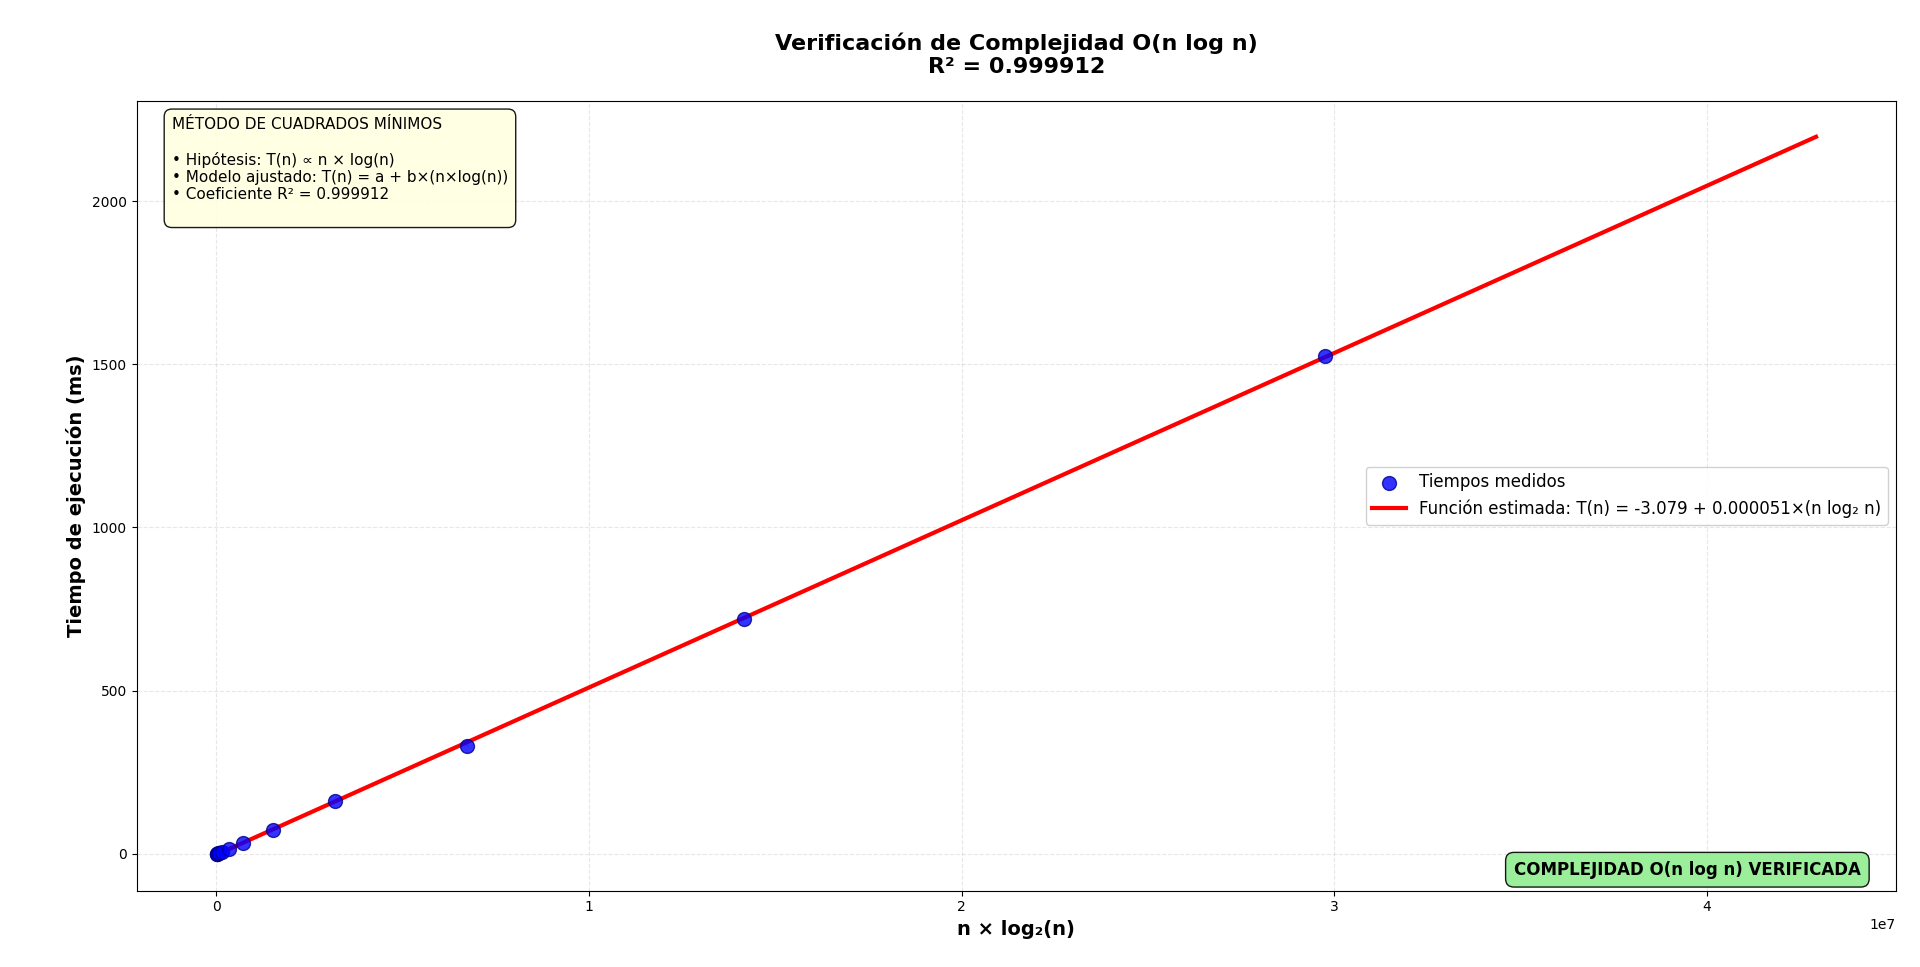
\includegraphics[width=0.8\textwidth]{./img/Figure_1.png}
    \caption{Gráfico de verificación de complejidad $O(n \log n)$}
\end{figure}

\subsection{Interpretacion de resultados}

Usamos el coeficiente de determinacion R²:

\begin{itemize}
    \item $R^2$ = 1.00: Ajuste perfecto (0\% de error)
    \item $R^2$ mayor 0.98: Excelente ajuste → Complejidad verificada
    \item $R^2$ mayor 0.95: Muy buen ajuste → Complejidad muy probable
    \item $R^2$ menor 0.90: Ajuste pobre → Resultados no concluyentes
\end{itemize}

\subsection{Conclusion}

Con un valor de $R^2 = 0.999912$, concluimos que la complejidad del algoritmo es $O(n \log n)$ debido a la alta calidad del ajuste.
\newpage
\section{Ejemplos ilustrativos del algoritmo greedy}
En los proximos dos ejemplos vamos a presentar casos border en donde se muestra que el algoritmo siempre nos da la solucion óptima

\subsection{Ejemplo 1: Todos los tiempos iguales}

\paragraph{Planteo del problema.}  
Tenemos la siguiente lista de batallas:
\begin{verbatim}
T_i,B_i
10,100
10,90
10,90
10,50
10,20
10,10
\end{verbatim}
Todas las batallas duran lo mismo ($t=10$). El objetivo es minimizar $\sum b_i F_i$.

\paragraph{Cálculo de razones y orden greedy.}  
Como $t_i=10$ para todas, la razón $\tfrac{b}{t}$ es proporcional al peso $b$.  
Ordenando de mayor a menor: 
\[
(10,100)\;\to\;(10,90)\;\to\;(10,90)\;\to\;(10,50)\;\to\;(10,20)\;\to\;(10,10).
\]

\paragraph{Cálculo del costo óptimo.}  
Los tiempos acumulados son $F=(10,20,30,40,50,60)$.  
Multiplicando cada $F_i$ por $b_i$:
\[
100\cdot10=1000,\;\;90\cdot20=1800,\;\;90\cdot30=2700,\;\;50\cdot40=2000,\;\;20\cdot50=1000,\;\;10\cdot60=600.
\]
La suma da:
\[
\sum b_i F_i = \boxed{9100}.
\]

\paragraph{Comparación con un orden incorrecto.}  
Si cambiamos el orden y ponemos primero $(10,90)$ y después $(10,100)$, obtenemos:
\[
\sum b_i F_i = 9200.
\]
Este valor es mayor que $9100$, mostrando que violar la regla empeora la solución.

\paragraph{Empates.}  
Las dos batallas $(10,90)$ tienen la misma razón $\tfrac{b}{t}=9$.  
Si las permutamos, el resultado total sigue siendo $9100$.  
Esto confirma que, ante empates, cualquier orden dentro del bloque es igualmente óptimo.

\subsection{Ejemplo 2: Empates no triviales en la razón}

\paragraph{Planteo del problema.}  
La lista de batallas es:
\begin{verbatim}
T_i,B_i
1,3
2,4
3,6
4,8
5,5
\end{verbatim}
Aquí los tiempos son distintos, y hay batallas con la misma razón $b/t$.

\paragraph{Cálculo de razones y orden greedy.}  
Las razones son:
\[
(1,3)\mapsto 3.0,\quad (2,4)\mapsto 2.0,\quad (3,6)\mapsto 2.0,\quad (4,8)\mapsto 2.0,\quad (5,5)\mapsto 1.0.
\]
El orden óptimo es:
\[
(1,3)\;\to\;(2,4)\;\to\;(3,6)\;\to\;(4,8)\;\to\;(5,5).
\]

\paragraph{Cálculo del costo óptimo.}  
Los tiempos acumulados son $F=(1,3,6,10,15)$.  
Contribuciones:
\[
3\cdot1=3,\;\;4\cdot3=12,\;\;6\cdot6=36,\;\;8\cdot10=80,\;\;5\cdot15=75.
\]
La suma da:
\[
\sum b_i F_i = \boxed{206}.
\]

\paragraph{Comparación con un orden incorrecto.}  
Si movemos $(5,5)$ delante de las batallas con razón $2.0$, obtenemos $F=(1,6,8,11,15)$ y un total de
\[
\sum b_i F_i = 251.
\]
Este valor es mayor que $206$, mostrando que romper el orden por $\tfrac{b}{t}$ empeora la solución.

\paragraph{Empates.}  
Las batallas $(2,4),(3,6),(4,8)$ tienen la misma razón $2.0$.  
Si se permutan entre ellas, por ejemplo $(4,8)\to(3,6)\to(2,4)$, el costo total sigue siendo $206$.  
Esto confirma que ante empates, cualquier permutación interna dentro del bloque mantiene la solución óptima.

\newpage
\section{Conclusión}
En este informe se busca ayudar a la ciudad de Ba Sing Se, una gran ciudad del Reino de la Tierra que se enfrenta al ejército de la Nación del Fuego. Nuestro objetivo es determinar en qué minutos realizar el contraataque para lograr la mayor cantidad posible de bajas enemigas.\\

Para resolver el problema se empleó una estrategia de \textit{Programación Dinámica}, que busca obtener la solución óptima mediante la descomposición del problema en subproblemas más pequeños. Almacenar ciertas soluciones intermedias permite simplificar los cálculos y evitar recomputaciones, generando así una dependencia entre decisiones: para poder obtener el minuto más eficiente es necesario considerar los minutos anteriores.\\

Durante el desarrollo del trabajo pudimos identificar tres parámetros principales: $n$, la cantidad de minutos de la batalla; $x$, la cantidad de enemigos por minuto; y $f(x)$, la cantidad de bajas en el minuto $x$ si se realiza el contraataque. Determinamos que la variable que define la complejidad del algoritmo es $n$, ya que determina la cantidad de veces que deben considerarse las soluciones. En el peor de los casos, nuestro algoritmo presentó una complejidad algorítmica de $O(n^2)$.\\

Finalmente, el algoritmo fue probado tanto con los casos de prueba proporcionados por la cátedra como con pruebas adicionales diseñadas por nosotros, incluyendo casos borde. Los resultados confirmaron la efectividad de la estrategia utilizada, validando así la pertinencia del enfoque adoptado. Este trabajo no solo permitió resolver el problema planteado, sino también afianzar el aprendizaje sobre el diseño, análisis y validación de algoritmos eficientes.


\newpage
\end{document}
